\chapter{How To Use the Template}
\label{cpt1}

This is the McKelvey School of Engineering LaTeX template for doctoral dissertations and master's theses. Using this template will help you produce a document compliant with the School's formatting guidelines.

Not every detail of the formatting guidelines can be encapsulated in a LaTeX template. For a narrative description of the guidelines, please see the School's Microsoft Word thesis template, which can be found as part of our \href{https://engineering.wustl.edu/offices-services/student-services/graduate-student-services/thesis-dissertation-submission.html}{thesis and dissertation submission procedures}. But you should be confident that using this LaTeX template will produce a document that complies with the School's requirements for spacing, margins, indentation, page numbering, chapter and section titles, and front matter formatting. Moreover, LaTeX's Computer Modern font family, which is the default for this template, is accepted as an alternative to the Times family specified in the Word template.

To use this template, you will need to review and edit two files: the top-level document (\texttt{thesis-main.tex}) and the front-matter file (\texttt{thesis-front.tex}).  You need not and \emph{should not} modify the class file \texttt{wuthesis.cls} at all.

\section{Top-Level Document}

The file \texttt{thesis-main.tex} is the top-level document for your thesis. At the top of this file, select the appropriate document type (master's thesis or doctoral dissertation) and then edit the fields that follow to provide the title, author, committee, and other information that will appear on the title page and in the abstract.  Note that the department/program name must be written exactly as described in the appendix of the Word template.

After filling in the fields at the top of the file, specify any LaTeX packages and configuration settings that should apply to the thesis document. You should then include the actual thesis chapters as shown using LaTeX's \texttt{\textbackslash include} command.  If your thesis has a preface, uncomment the two preface lines and provide the preface as a separate \texttt{.tex} file. If your thesis has appendices, include these after the \texttt{\textbackslash appendix} line at the bottom of the file to ensure that they will be correctly numbered and formatted.

Finally, \texttt{thesis-main.tex} creates the bibliography for your document~\cite{Lovecraft1928} using BibTeX. If desired, you can change the bibliography style to whatever is appropriate for your discipline. Reference information may be added to the provided \texttt{.bib} file.

\section{Front Matter}

The file \texttt{thesis-front.tex} creates the front-matter sections of the thesis.  Much of the front matter is generated automatically from the fields you provide in \texttt{thesis-main.tex}, but there are a few sections that require you to provide your own text.  They are:

\begin{itemize}

\item List of Abbreviations (\textit{optional}) -- uncomment the indicated lines in the front-matter file and provide a \texttt{.tex} file listing all your abbreviations and notation. This template uses the LaTeX \texttt{nomencl} package, which formats the list for you; see that package's documentation for details.

\item Acknowledgments (\textbf{required}) -- write the text of your acknowledgments page in the provided \texttt{\textbackslash thesisacknowledgments} environment.

\item Abstract (\textbf{required}) -- write the text of your abstract in the provided \texttt{\textbackslash thesisabstract} environment.

\item Dedication (\textit{optional}) -- if you wish to produce a dedication page separate from your acknowledgments, uncomment the \texttt{\textbackslash thesisdedicationpage} environment and write a brief dedication.

\end{itemize}
\emph{You should not add to or modify the contents of the front-matter document}, other than filling in the items listed above.

\section{Advice on Figures and Tables}

When including a figure or table in your thesis, remember that the caption will be copied verbatim into the List Figures or List of Tables in the front matter.  This means that you will potentially end up with a paragraph for each entry in those lists, which looks odd.

% Note: use the bracketed version of caption, i.e. \caption[short-version]{text} to produce a separate, shortened version of the caption for the LoF or LoT.

\begin{figure}
    \centering
    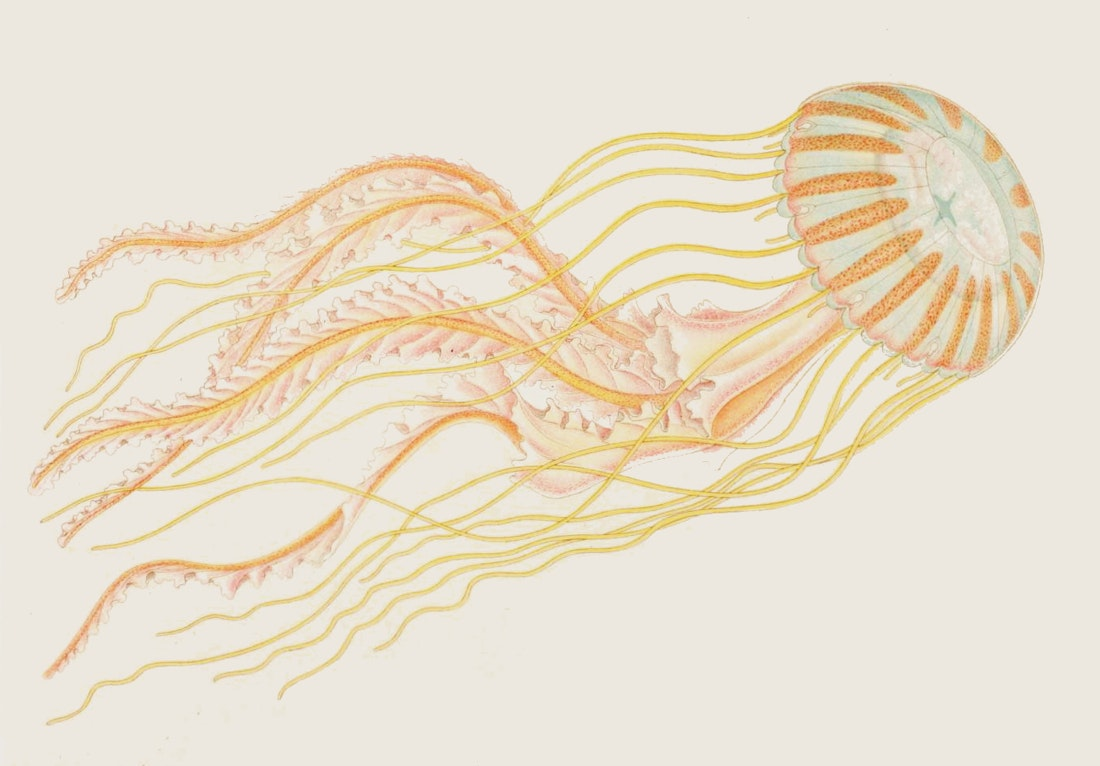
\includegraphics[width=0.6 \textwidth] {jellyfish}
    \caption[A Picture of a Jellyfish]{Jellyfish, from A.~G. Meyer, \textit{Medusae of the World}, 1910. It is venomous and squishy.}
    \label{fig:jelly}
\end{figure}

You can supply a \emph{short caption} for a figure or table that replaces the full caption in the front matter.  To do this, include the short caption in square brackets after the \texttt{\textbackslash caption} command and before the regular caption, as shown in the LaTeX source for Figure~\ref{fig:jelly} and Table~\ref{tab:fish}.

\begin{table}[b]
\centering
    \caption[A Table of Fish]{Number and color of assorted fish.  Here, fishy fishy fish!}
    \label{tab:fish}
    \begin{tabular}{|c|c|}
    \hline
         One Fish & Two Fish  \\
         Red Fish & Blue Fish \\
    \hline
    \end{tabular}
\end{table}

